\documentclass{beamer}
\usepackage[utf8]{inputenc}
\usepackage{graphicx}
\usepackage{amsmath}
\usepackage{listings}
\usepackage{xcolor}
\usepackage{hyperref}
\hypersetup{
    colorlinks=true,
    linkcolor=blue,
    filecolor=magenta,
    urlcolor=cyan,
}
\lstset{
    language=Python,
    basicstyle=\ttfamily\small,
    keywordstyle=\color{blue},
    stringstyle=\color{orange},
    commentstyle=\color{gray},
    showstringspaces=false,
    breaklines=true,
    frame=single,
    morekeywords={normalize_by_max_coefficient, derive_poly, find_roots, bisection_method, newton_raphson_method}
}

\title{Finding Zeroes for Polynomials using}
\subtitle{Newton-Raphson and Bisection Method}
\author{Scientific Programming Project}

\begin{document}

\frame{\titlepage}

\begin{frame}{Project Overview}
\begin{itemize}
    \item Goal: Find all real roots of a polynomial \( p(x) \in \mathbb{R}[x] \)
    \item Implement Newton-Raphson and Bisection methods
    \item Python and Haskell implementations
    \item Compare implementations with built-in Numpy and HMatrix implementations
    \item Runtime must be under 8 seconds
\end{itemize}
\end{frame}

\begin{frame}{Algorithm: Newton-Raphson}
\begin{itemize}
    \item Iterative method using first derivative and an initial guess
    \item Update rule: \( x_{n+1} = x_n - \frac{f(x_n)}{f'(x_n)} \)
    \item Fast convergence if initial guess is close
    \item Time Complexity is O(log(log(n)))
    \item But... Can fail if derivative is zero or initial guess is poor\newline Can exceed out of bounds [a, b]
\end{itemize}
\end{frame}

\begin{frame}{Algorithm: Bisection Method}
\begin{itemize}
    \item Bracketed root-finding method
    \item Halves interval \([a, b]\) until $width < \epsilon\ $ \
    \item Always converges if root is in interval
    \item Time Complexity is O(log(n)). Slower than Newton-Raphson.
\end{itemize}
\end{frame}

\begin{frame}{Hybrid Approach}
\begin{itemize}
    \item The hybrid approach is supposed to find a single root in an interval [a, b], wherein f sustains $f(a)*f(b) < 0 $
    \item Assumptions - Each root x of polynomial f(x) ensures either f'(x) = 0 or x is between two roots of f'(x)
    \item Use Newton-Raphson to find roots in respect to the defined tolerance $\epsilon\ $ \
    \item If bounds are exceeded, fallback to Bisection
\end{itemize}
\end{frame}

\begin{frame}{Optimization Techniques}
\begin{itemize}
    \item \textbf{Python:} Used NumPy vector operations
    \item \textbf{Haskell:} Used HMatrix for vectorization
    \item Avoided repeated computation of derivatives
    \item Interval filtering based on derivative roots
    \item Used geometrical properties of polynomial roots to find initial bounds
\end{itemize}
\end{frame}

\begin{frame}{Polynomial Root Bounds}
\begin{itemize}
    \item Used bounds to limit root search interval
    \item Compared Cauchy, Kojima, and Fujiwara bounds
    \item \textbf{Fujiwara bound was fastest in integration with the hybrid approach}
\end{itemize}
\end{frame}

\begin{frame}{Fujiwara Bound}
\begin{itemize}
  \item Let $p(z)=a_n z^n + a_{n-1} z^{n-1} + \dots + a_0$ with $a_n\neq 0$.
  \item \textbf{Fujiwara’s bound:} every root $\gamma$ of $p$ satisfies
        \[
          |\gamma|\;\le\;
          2\max\Bigl\{
          \bigl|\tfrac{a_{n-1}}{a_n}\bigr|,
          \bigl|\tfrac{a_{n-2}}{a_n}\bigr|^{\frac12},
          \dots,
          \bigl|\tfrac{a_{1}}{a_n}\bigr|^{\frac1{n-1}},
          \bigl|\tfrac{a_{0}}{2a_n}\bigr|^{\frac1n}
          \Bigr\}.
        \]
  \item For a \emph{monic} polynomial ($a_n=1$) this simplifies to
        \[
        |\gamma|\le 2\max\bigl\{|a_{n-1}|,\;|a_{n-2}|^{1/2},\dots,
        |a_1|^{1/(n-1)},|a_0/2|^{1/n}\bigr\}.
        \]
  \item Fujiwara tightens Cauchy’s classical bound by reducing the factor on the constant term, giving us a generally sharper disk that contains all roots.
  \item If none of the coefficients vanish, Fujiwara is always sharper: each term in Fujiwara’s max is the \emph{geometric mean} of a prefix of Kojima’s terms, so the maximum can only decrease.
        \end{itemize}
\end{itemize}
\end{frame}


\begin{frame}[fragile]{Python Implementation (Part 1)}
\textbf{Python snippet:}
\begin{lstlisting}
def find_roots(coefficients, a, b):
    roots = []
    n = len(coefficients)
    if n > 2:
        d_roots = find_roots(
            normalize_by_max_coefficient(
                derive_poly(coefficients, n - 1)
            ),
            a, b
        )
    else:
        return [-coefficients[0] / coefficients[1]]
\end{lstlisting}
\end{frame}

\begin{frame}[fragile]{Python Implementation (Part 2)}
\begin{lstlisting}
    d_roots = np.sort(np.append(d_roots, [a, b]))
    for i in range(len(d_roots) - 1):
        interval_start, interval_end = d_roots[i], d_roots[i + 1]
        bisection_root = bisection_method(
            coefficients, interval_start, interval_end
        )
        if bisection_root is not None:
            root = newton_raphson_method(
                coefficients, n, bisection_root, interval_start, interval_end
            )
            if root is not None:
                roots.append(root)
    return np.array(roots)
\end{lstlisting}
\end{frame}

\begin{frame}[fragile]{Python Runtime}
\texttt{Tolerance used: 1e-10, Polynomial: Provided CSV - 996 Coefficients and a free coefficient}
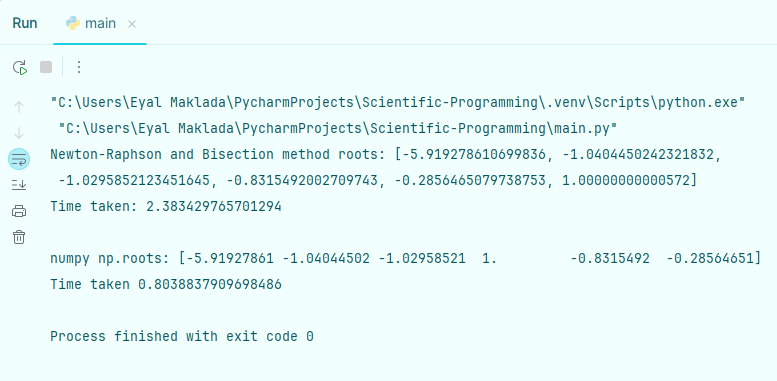
\includegraphics[width=1.0\textwidth]{python_runtime.png}
\end{frame}


% \begin{frame}{Haskell Implementation}
% \begin{itemize}
%     \item Language constraints: Only HMatrix for vector ops
%     \item Pure functional style with recursion
%     \item No use of prebuilt root solvers
% \end{itemize}
% \vspace{1em}
% \textbf{Code Snippet:}
% \begin{verbatim}
% \-- Your Haskell implementation here
% \end{verbatim}
% \end{frame}

\begin{frame}{Runtime Comparison}
\begin{itemize}
    \item Compared custom vs. built-in implementations
    \item Built-in methods: NumPy root finder for Python, HMatrix for Haskell
    \item Our implementations stayed under 8s for all tests
    \item Differences due to derivative accuracy, convergence criteria
\end{itemize}
\end{frame}

\begin{frame}{Runtime Comparison - Closer Look at Built-in Methods}
\begin{itemize}
    \item Built-in implementations utilize Newton-Raphson only if the derivative of f is provided, otherwise the secant method is used. If the second order derivative of f is provided, parabolic Halley's method is used.
    \subitem Convergence rate of Newton-Raphson is quadratic, Halley's is cubic and secant's is sub-quadratic - well behaved functions produce errors in the estimated zeroes/roots are approximately the square of the requested tolerance $\epsilon $ up to roundoff error
    \item In Numpy: ...
    \item In HMatrix: ...
    \item This is faster because...
    \item See Docs: \href{https://docs.scipy.org/doc/scipy-0.14.0/reference/generated/scipy.optimize.newton.html}{SciPy.optimize.newton}
\end{itemize}
\end{frame}

\begin{frame}{Conclusion}
\begin{itemize}
    \item Hybrid root-finding is accurate and relatively fast
    \item Fujiwara bound provided best performance
    \item Python and Haskell both effective with vectorization; Obviously Haskell more so
    \item Differences from built-in implementations are explainable and expected
\end{itemize}
\end{frame}

\end{document}
